\chapter{Recombination and the thermal history}\label{ch:recombination}
\chapterstatus{written}{2026-11-14}

Before recombination photons, electrons and nuclei form a plasma in which Thomson scattering is so frequent that
photons and baryons move as one fluid. When the universe has cooled enough for the electrons to bind into atoms the
scattering stops and the photons stream freely towards us as the CMB. This chapter describes the calculation of the
free-electron fraction $X_e(x)$, the baryon temperature, reionization, and the derived optical depth $\tau$,
visibility function $\gt$ and sound horizon, which set where and how the CMB photons last scattered and the scale of
the baryon acoustic oscillations.

\begin{modulebox}{Cosmology/Recombination}
\file{Cosmology/Recombination/RecombinationHistory.h/.cpp}: the class \cls{RecombinationHistory} (namespace
\nsp{FML::COSMOLOGY}), built on a \cls{BackgroundCosmology} (\cref{ch:background}); helium from BBN in
\file{Cosmology/Background/BBN.h}.\par
Parameters: the \code{Recombination} section of the Einstein--Boltzmann solver's parameter file
(\file{Cosmology/EinsteinBoltzmannSolver/params/default.ini}). Physics, validation and figures: the solver report
\file{Cosmology/EinsteinBoltzmannSolver/report/paper.pdf}, Secs.~II and IX.
\end{modulebox}

\section{Definitions}

The number density of hydrogen nuclei (free or bound) is $n_H=(1-Y_p)\rho_b/m_H\propto a^{-3}$, with $Y_p$ the
primordial helium mass fraction (given, default $0.245$, or from BBN, \cref{ch:background}). Helium contributes
$f_{\rm He}=n_{\rm He}/n_H$ nuclei per hydrogen nucleus: $f_{\rm He}=Y_p/[4(1-Y_p)]$ in the Peebles model and
$Y_p/[3.9715(1-Y_p)]$ (the true helium-to-hydrogen mass ratio) in RECFAST. The free-electron fraction is
\begin{equation}
X_e=\frac{n_e}{n_H}=x_{\rm H}+f_{\rm He}\,(x_{\rm He^+}+2x_{\rm He^{++}}),
\end{equation}
which is $1+2f_{\rm He}$ when everything is ionized.

\section{Saha equilibrium}

At early times $e^-+p\leftrightarrow{\rm H}+\gamma$ is much faster than the expansion and in chemical equilibrium.
For non-relativistic Maxwell--Boltzmann species the chemical potentials cancel in $n_en_p/n_{\rm H}$, leaving the
binding energy $\epsilon_0=13.6$\,eV, and similarly for the two ionization stages of helium:
\begin{equation}
\frac{n_ex_{\rm H^+}}{1-x_{\rm H^+}}=F\,e^{-\epsilon_0/k_BT_b},\qquad
\frac{n_ex_{\rm He^+}}{x_{\rm He^0}}=4F\,e^{-\chi_0/k_BT_b},\qquad
\frac{n_ex_{\rm He^{++}}}{x_{\rm He^+}}=F\,e^{-\chi_1/k_BT_b},
\label{eq:rec-saha}
\end{equation}
with $F=(m_ek_BT_b/2\pi\hbar^2)^{3/2}$, $\chi_0=24.59$\,eV and $\chi_1=54.4$\,eV. The three equations and
$n_e=n_H[x_{\rm H^+}+f_{\rm He}(x_{\rm He^+}+2x_{\rm He^{++}})]$ are solved together by root finding in $\ln n_e$.
Because there are $\sim10^9$ photons per baryon, the Wien tail of the Planck spectrum keeps hydrogen ionized until
$\epsilon_0/k_BT\approx40$--$50$, i.e.\ $z\approx1300$.

\section{The Peebles model}

Direct recombinations to the ground state emit a photon that ionizes another atom, and Lyman-$\alpha$ photons from
$2p\to1s$ are immediately reabsorbed; only the two-photon decay $2s\to1s$ ($\Lambda_{2s\to1s}=8.227$\,s$^{-1}$) and the
redshifting of Lyman-$\alpha$ photons out of the line lead to the ground state. Peebles' effective three-level atom
\cite{Peebles1968} gives
\begin{equation}
\frac{\dd X_e}{\dd x}=\frac{C_r(T_b)}{H}\left[\beta(T_b)(1-X_e)-n_H\alpha^{(2)}(T_b)X_e^2\right],\qquad
C_r=\frac{\Lambda_{2s\to1s}+\Lambda_\alpha}{\Lambda_{2s\to1s}+\Lambda_\alpha+\beta^{(2)}},
\label{eq:rec-peebles}
\end{equation}
with the rates of Callin \cite{Callin2006}:
\begin{gather}
\alpha^{(2)}=\frac{64\pi}{\sqrt{27\pi}}\frac{\alpha^2\hbar^2}{m_e^2c}\sqrt{\frac{\epsilon_0}{k_BT_b}}\,\phi_2(T_b),\quad
\phi_2=0.448\ln\frac{\epsilon_0}{k_BT_b},\qquad \beta=\alpha^{(2)}Fe^{-\epsilon_0/k_BT_b},\\
\beta^{(2)}=\beta\,e^{3\epsilon_0/4k_BT_b},\qquad
\Lambda_\alpha=\frac{H(3\epsilon_0)^3}{(8\pi)^2(\hbar c)^3n_{1s}},\qquad n_{1s}=(1-X_e)n_H .
\end{gather}
$C_r$ is the probability that an atom in $n=2$ reaches the ground state before it is ionized again. Early on
$C_r\ll1$ and recombination lags behind Saha equilibrium; late, $n_e\alpha^{(2)}<H$ and $X_e$ freezes out at
$\sim2\times10^{-4}$. A fudge factor on $\alpha^{(2)}$ (\param{rec_peebles_fudge}; 1.14 is RECFAST's original value
\cite{Seager1999}) is available. In this model helium stays in Saha equilibrium given the electron density.

\section{RECFAST}

The default model (\param{recombination} \code{= recfast}) is RECFAST 1.5
\cite{Seager1999,Wong2008,RubinoMartin2010}, which reproduces multi-level atom calculations to $\sim0.1\%$ in $X_e$
with three ODEs for $x_{\rm H}=n_{\rm HII}/n_H$, $x_{\rm He}=n_{\rm HeII}/n_{\rm He}$ and $T_b$. For hydrogen,
\begin{gather}
\frac{\dd x_{\rm H}}{\dd z}=\frac{X_ex_{\rm H}n_H\alpha_{\rm H}-\beta_{\rm H}(1-x_{\rm H})e^{-h\nu_{{\rm Ly}\alpha}/k_BT_b}}{H(1+z)}\,C_{\rm H},\\
C_{\rm H}=\frac{1+K_{\rm H}\Lambda_{2s1s}n_{1s}}{F_{\rm H}^{-1}(1+K_{\rm H}\Lambda_{2s1s}n_{1s})+K_{\rm H}\beta_{\rm H}n_{1s}},\qquad
K_{\rm H}=\frac{\lambda_{{\rm Ly}\alpha}^3}{8\pi H}\left[1+\sum_{i=1}^2A_ie^{-[(\ln(1+z)-z_i)/w_i]^2}\right],
\end{gather}
with the case-B coefficient of P\'equignot et al.\ \cite{Pequignot1991},
$\alpha_{\rm H}=10^{-19}F_{\rm H}\,at^b/(1+ct^d)$\,m$^3$\,s$^{-1}$, $t=T_b/10^4$\,K, the photoionization rate
$\beta_{\rm H}=\alpha_{\rm H}(2\pi m_ek_BT_b/h^2)^{3/2}e^{-h\nu_{2s}/k_BT_b}$, the fudge factor
$F_{\rm H}=1.125$ (\param{rec_recfast_fudge_H}) and the double-Gaussian correction to the Lyman-$\alpha$ escape of
RECFAST 1.5. Neutral helium uses the same form for the He\,I singlet system (2$^1$S two-photon rate $51.3$\,s$^{-1}$,
recombination rate of Verner and Ferland \cite{Verner1996}) with two additions that speed up helium recombination:
the escape of 2$^1$P photons through continuum absorption by neutral hydrogen (calibrated by $F_{\rm He}=0.86$,
\param{rec_recfast_fudge_He}) and recombination through the triplet 2$^3$P state. Einstein coefficients, energy
levels and fits are those of RECFAST 1.5 as used in CLASS.

\section{Baryon temperature}

Compton scattering off the CMB photons keeps the gas at the photon temperature, while adiabatic expansion alone
would cool it as $a^{-2}$:
\begin{equation}
\frac{\dd T_b}{\dd x}=-2T_b+\frac{8\sigma_Ta_RT_\gamma^4}{3m_ecH}\,\frac{X_e}{1+f_{\rm He}+X_e}\,(T_\gamma-T_b).
\end{equation}
The coupling is $\sim10^6H$ at recombination, so $T_b=T_\gamma$ until $z\sim500$. With
\param{rec_evolve_Tb} \code{= false}, $T_b=T_\gamma$ throughout.

\section{Reionization}

The intergalactic medium was reionized by the first stars and quasars. The library uses the CAMB/CLASS
parameterization (\code{reio_camb}) \cite{Lewis2008},
\begin{gather}
X_e=X_e^{\rm rec}+\left(1+f_{\rm He}-X_e^{\rm rec}\right)\frac{1+\tanh\frac{y_{\rm re}-y}{\Delta y}}{2}
+f_{\rm He}\,\frac{1+\tanh\frac{z_{\rm He}-z}{\Delta z_{\rm He}}}{2},\\
y=(1+z)^{3/2},\qquad \Delta y=\tfrac32(1+z_{\rm re})^{1/2}\Delta z,
\end{gather}
which reionizes hydrogen and the first helium electron at $z_{\rm re}$ (\param{z_reion}, width
\param{delta_z_reion}) and the second helium electron at $z_{\rm He}$ (\param{z_He_reion},
\param{delta_z_He_reion}). The optical depth to reionization is reported, as CLASS's $\tau_{\rm reio}$, from $z=0$ to
$z_{\rm re}+8\Delta z$; \code{tau_reionization_model(z_re)} gives the optical depth of the tanh steps alone without a
solve, which the samplers use to parameterize by $\tau$ instead of $z_{\rm re}$.

\section{Optical depth, visibility and the sound horizon}

A photon scatters at the rate $n_e\sigma_Tc$. The optical depth back to $x$ and the visibility function are
\begin{equation}
\tau(x)=\int_x^0\frac{cn_e\sigma_T}{H}\dd x',\qquad \tau'=-\frac{cn_e\sigma_T}{H},\qquad
\gt(x)=-\tau'e^{-\tau},\qquad \int\gt\,\dd x=1 .
\end{equation}
$\gt$ is the probability density that a photon observed today last scattered at $x$; the last-scattering surface
($\tau=1$, $z_*\approx1090$) has a width $\Delta z\approx200$. Before decoupling the photon--baryon fluid has the sound
speed $c_s=c/\sqrt{3(1+R_b)}$ with $R_b=3\rho_b/(4\rho_\gamma)$; the code uses the inverse $R=1/R_b=4\Om_\gamma/(3\Om_ba)$,
as in the perturbation equations, so
\begin{equation}
r_s(x)=\int_{-\infty}^x\frac{c_s}{\Hp}\,\dd x',\qquad c_s=c\sqrt{\frac{R}{3(1+R)}} .
\end{equation}
The baryons are released later than the photons, at the drag epoch where the drag optical depth
$\tau_d(x)=-\int_x^0\tau'R\,\dd x'$ reaches unity ($z_d\approx1060$). $r_s(z_d)\approx147$\,Mpc is the BAO scale.

\begin{implementation}
\begin{itemize}
\item The solution is computed on \param{rec_n_points} $=40\,000$ points in $x\in[\code{rec_x_start},0]=[-20,0]$.
\item \emph{RECFAST}: three phases as in RECFAST itself --- Saha for H$^+$, He$^+$ and He$^{++}$ together while
      everything is close to equilibrium; the helium ODE with hydrogen in Saha equilibrium once $x_{\rm He}<0.995$
      ($z\approx2900$); the full $(x_{\rm H},x_{\rm He},T_b)$ system once $x_{\rm H}<0.995$ ($z\approx1600$). The switch
      leaves a small kink in $\dd X_e/\dd x$ where the visibility is $10^{-13}$ of its maximum.
\item \emph{Peebles}: Saha while $x_{\rm H}>$ \param{rec_Xe_saha_limit} $=0.99$, then the Peebles equation with
      helium from Saha given $x_{\rm H}$; \param{rec_helium} \code{= false} keeps helium neutral.
\item The system is stiff (rates $\gg H$), so it is integrated with GSL's implicit multistep BDF method. $X_e$ is
      splined in $\ln X_e$. $\tau$ is integrated backwards from $\tau(0)=0$, $\tau'$ is analytic from $n_e$, and $\tau''$,
      $\gt'$, $\gt''$ (needed by the source functions) come from splines.
\item Outputs: \code{Xe_of_x}, \code{ne_of_x}, \code{tau_of_x} and its derivatives, \code{g_tilde_of_x} and
      derivatives, \code{Tb_of_x}, \code{R_of_x}, \code{sound_horizon_of_x}, and the epochs (\code{x_last_scattering}, \code{x_visibility_peak}, \code{x_Xe_half}, recombination
      ($X_e=0.1$) and the drag epoch). \code{output()} writes the table \file{recombination.txt}. The whole calculation
      takes $\approx0.35$\,s.
\end{itemize}
\end{implementation}

\begin{figure}[htbp]
\centering
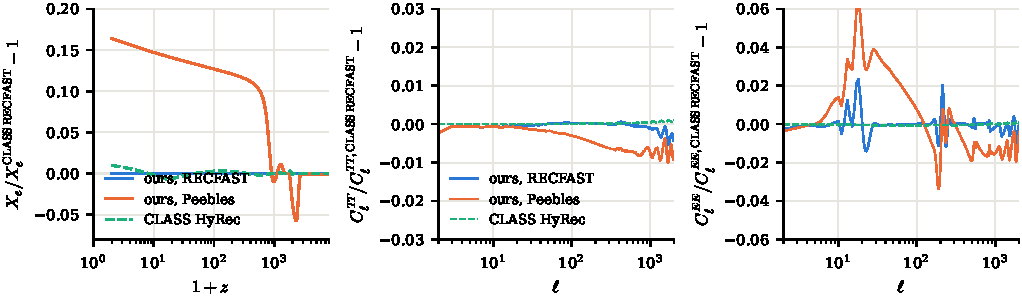
\includegraphics[width=\textwidth]{recfast}
\caption{\emph{Left:} $X_e(z)$ without reionization relative to CLASS run with RECFAST, for RECFAST (blue) and the
Peebles model (orange); dashed: CLASS with HyRec. \emph{Middle, right:} the unlensed TT and EE spectra relative to
CLASS with RECFAST. From the solver report.}
\label{fig:rec-recfast}
\end{figure}

\begin{validation}
\begin{itemize}
\item Plateaus: $X_e=1+2f_{\rm He}$ before helium recombination, $1+f_{\rm He}$ on the He$^+$ plateau; with $Y_p=0$ the
      helium solver reproduces the hydrogen-only code exactly.
\item $\int\gt\,\dd x=1$ to machine precision; $\tau'$, $\tau''$, $\gt'$, $\gt''$ against finite differences;
      $r_s$ against an independent quadrature; $T_b=T_\gamma$ early and $T_b\propto a^{-2}$ late.
\item The reionization optical depth agrees with the analytic integral for instantaneous reionization.
\item Against CLASS with RECFAST: $X_e$ to $3.3\times10^{-4}$ for $0\le z\le8000$ (both helium recombinations
      included), $z_*$ and $r_s(z_*)$ to $10^{-6}$ (\cref{fig:rec-recfast}). The rms difference of the unlensed TT
      from CLASS is $0.048\%$ for $30\le\ell\le1000$ with RECFAST against $0.64\%$ with the Peebles model.
\end{itemize}
\end{validation}

\begin{cppcode}[Recombination on its own]
#include <FML/Cosmology/Recombination/RecombinationHistory.h>
using namespace FML::COSMOLOGY;
CosmologyParameters params = CosmologyParameters::Planck2018Baseline();
BackgroundCosmology cosmo(params);
cosmo.solve();
RecombinationHistory rec(cosmo);
rec.solve();
rec.info();                               // z_*, r_s, z_drag, tau_reio, ...
double g = rec.g_tilde_of_x(-7.0);        // visibility at x = -7
rec.output("data/recombination.txt");
\end{cppcode}
